Chương này trình bày nền tảng lý thuyết của đề tài, từ cơ chế ARQ/HARQ cơ bản đến đặc tính kênh vệ tinh và vấn đề pipeline trong mạng NTN.

\subsection{Từ ARQ đến HARQ}

\subsubsection{ARQ cơ bản}

Automatic Repeat reQuest (ARQ) là cơ chế sửa lỗi lớp liên kết dựa trên phản hồi: bên thu gửi ACK (nhận đúng) hoặc NACK (nhận sai), bên phát phát lại nếu nhận NACK. Có ba biến thể chính: Stop-and-Wait (SAW), Go-Back-N (GBN), và Selective Repeat (SR)~\cite{proakis2008}. Trong 5G NR, RLC ARQ sử dụng cơ chế SR với cửa sổ có thể cấu hình~\cite{ts38321}.

\textbf{Hạn chế của ARQ thuần túy:} Mỗi lần phát lại là độc lập, toàn bộ năng lượng của lần phát trước bị lãng phí. Hơn nữa, bên thu phải chờ lần phát mới hoàn toàn để giải mã, thay vì tận dụng tín hiệu đã nhận (dù có lỗi) để hỗ trợ giải mã.

\subsubsection{HARQ: kết hợp mã hóa và tái phát}

HARQ (Hybrid ARQ) kết hợp FEC (Forward Error Correction) với ARQ bằng cách lưu trữ tín hiệu nhận được từ các lần phát trước trong bộ đệm HARQ (Chase Buffer) và kết hợp chúng trước khi giải mã. Điều này biến mỗi lần phát lại thành nguồn thông tin bổ sung thay vì thay thế hoàn toàn lần trước.

Hai sơ đồ kết hợp chính trong 5G NR~\cite{ts38212}:

\paragraph{Chase Combining (CC-HARQ):} Mỗi lần phát lại gửi cùng một khối bit mã hóa (cùng RV = 0). Bộ thu kết hợp bằng Maximum Ratio Combining (MRC), cộng SNR tức thời:
\begin{equation}\label{eq:cc_snr}
    \gamma_{\text{eff}}^{(n)} = \sum_{i=1}^{n} \gamma_i
\end{equation}
trong đó $\gamma_i = |h_i|^2 \cdot (E_s/N_0)$ là SNR tức thời lần phát thứ $i$~\cite{chase1985}.

\paragraph{Incremental Redundancy (IR-HARQ):} Mỗi lần phát lại gửi các bit dư thừa mới (RV khác nhau: \{0, 2, 3, 1\} theo TS 38.212~\cite{ts38212}), lấy từ vùng khác nhau của circular buffer LDPC. Bộ thu tích lũy thông tin tương hỗ (mutual information):
\begin{equation}\label{eq:ir_mi}
    I^{(n)} = m_{TX} \sum_{i=1}^{n} \log_2\!\left(1 + \frac{\gamma_i}{\Delta}\right)
\end{equation}
trong đó $m_{TX} = k/r$ là số bit mã hóa mỗi lần phát (chuẩn hóa), $\Delta$ là khoảng cách thực thi LDPC~\cite{hagenauer1988}.

\subsubsection{Lợi thế của IR so với CC}

Từ phương trình (\ref{eq:cc_snr}) và (\ref{eq:ir_mi}), thông tin tương hỗ của CC và IR lần lượt là:
\begin{align}
    I_{\text{CC}}^{(n)} &= m_{TX} \cdot \log_2\!\left(1 + \frac{\sum_i \gamma_i}{\Delta}\right) \label{eq:mi_cc}\\
    I_{\text{IR}}^{(n)} &= m_{TX} \cdot \sum_{i=1}^{n} \log_2\!\left(1 + \frac{\gamma_i}{\Delta}\right) \label{eq:mi_ir}
\end{align}

Áp dụng bất đẳng thức Jensen cho hàm lõm $\log_2(1 + x/\Delta)$:
\begin{equation}\label{eq:jensen}
    \sum_{i=1}^{n} \log_2\!\left(1 + \frac{\gamma_i}{\Delta}\right) \;\geq\; \log_2\!\left(1 + \frac{\sum_i \gamma_i}{\Delta}\right)
\end{equation}

Do đó $I_{\text{IR}}^{(n)} \geq I_{\text{CC}}^{(n)}$ với dấu bằng khi và chỉ khi $n = 1$ (lần phát đầu tiên giống nhau) hoặc tất cả $\gamma_i$ bằng nhau. Đây là nền tảng lý thuyết cho việc IR luôn vượt trội hơn CC từ lần phát thứ hai trở đi.

\subsection{Kênh vệ tinh -- Mặt đất: Mô hình Rician}

\subsubsection{Phân phối Rician và hệ số K}

Kênh Land Mobile Satellite (LMS) trong điều kiện tầm nhìn thẳng được mô tả bởi phân phối Rician. Hệ số kênh phức có dạng~\cite{tr38811}:
\begin{equation}\label{eq:rician_h}
    h = \underbrace{\sqrt{\frac{K}{K+1}} e^{j\phi}}_{\text{thành phần LOS}} + \underbrace{\sqrt{\frac{1}{K+1}} \cdot h_{\text{scatter}}}_{\text{thành phần tán xạ}}
\end{equation}
trong đó $K$ là hệ số Rician (tỷ lệ công suất LOS/tán xạ), $\phi \sim \mathcal{U}[0, 2\pi)$ là pha ngẫu nhiên của LOS, $h_{\text{scatter}} \sim \mathcal{CN}(0,1)$. Xây dựng này đảm bảo $\mathbb{E}[|h|^2] = 1$ chính xác.

SNR tức thời: $\gamma = |h|^2 \cdot (E_s/N_0)$. Phân phối của $|h|^2$ là chi-squared phi tâm bậc tự do 2, nghịch đảo non-centrality $2K$:
\begin{equation}\label{eq:rician_cdf}
    F_{|h|^2}(x) = 1 - Q_1\!\left(\sqrt{2K},\, \sqrt{2(K+1)x}\right)
\end{equation}
trong đó $Q_1(\cdot,\cdot)$ là hàm Marcum Q bậc 1~\cite{proakis2008}. Trong mô phỏng, đây tương đương với phân phối ncx2 (df = 2, nc = 2K).

\subsubsection{Tham số kênh NTN}

TR 38.811 Mục 6.7.1 xác định mô hình kênh LMS cho NTN với các tham số:

\begin{table}[H]
    \centering
    \caption[Tham số kênh NTN theo TR 38.811]{\bfseries\fontsize{12pt}{0pt}\selectfont Tham số kênh LMS NTN điển hình (TR 38.811 Mục 6.7.1)}
    \label{tab:channel_params}
    \begin{tabularx}{0.9\textwidth}{
    | >{\centering\arraybackslash}X
    | >{\centering\arraybackslash}X
    | >{\centering\arraybackslash}X |}
    \hline
    \bfseries Tham số & \bfseries Ký hiệu & \bfseries Giá trị \\\hline
    Hệ số Rician & $K_{\text{dB}}$ & 15 dB \\\hline
    Tần số sóng mang & $f_c$ & 20 GHz (Ka-band) \\\hline
    Tốc độ UE & $v$ & 50 km/h \\\hline
    Mô hình kênh & -- & Rician phẳng, LMS \\\hline
    \end{tabularx}
\end{table}

\subsubsection{Thời gian kết hợp và fading}

Thời gian kết hợp kênh (Doppler coherence time)~\cite{tuninato2025}:
\begin{equation}\label{eq:coherence}
    T_c \approx \frac{0{,}423}{f_d}, \quad f_d = \frac{v}{c} \cdot f_c
\end{equation}
Với $v = 50$ km/h, $f_c = 20$ GHz: $f_d \approx 926$ Hz, $T_c \approx 0{,}46$ ms. So sánh với $T_{\text{slot}} = 0{,}5$ ms (SCS 30 kHz), kênh thay đổi gần bằng một slot -- tức là các lần phát lại HARQ liên tiếp có thể gặp các thực hiện kênh gần độc lập.

\subsection{Pipeline HARQ trong NTN}

\subsubsection{Cơ chế pipeline HARQ}

Trong 5G NR, giao thức HARQ sử dụng N tiến trình song song (N-process pipeline) để duy trì truyền liên tục khi chờ ACK/NACK~\cite{ts38321}. Mỗi tiến trình $p_i$ truyền độc lập: bên phát gửi khối dữ liệu (TB) ở slot $t$, bên thu xử lý và trả ACK/NACK sau một khoảng thời gian bằng RTT; chỉ khi nhận được phản hồi, bên phát mới được dùng lại tiến trình đó. Nếu số tiến trình N không đủ để lấp đầy khoảng trống chờ, bộ phát phải dừng lại -- gọi là \textit{pipeline stall}.

\begin{figure}[H]
\centering
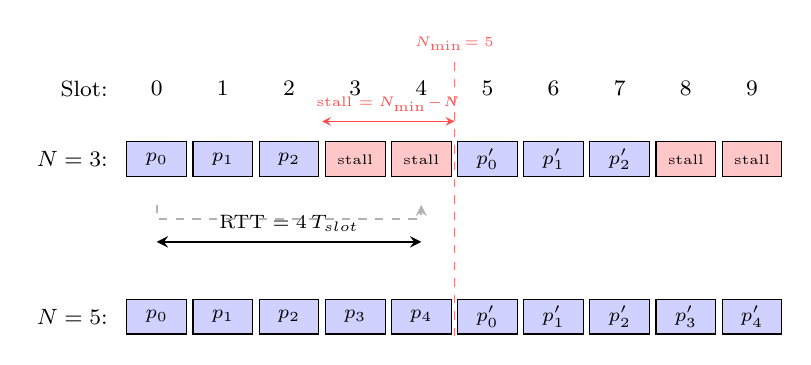
\begin{tikzpicture}[
    tx/.style={draw, fill=blue!18, minimum width=0.76cm, minimum height=0.44cm,
               font=\scriptsize, inner sep=0pt},
    st/.style={draw, fill=red!22, minimum width=0.76cm, minimum height=0.44cm,
               font=\scriptsize, inner sep=0pt},
    >=stealth
]
\def\W{0.84}
% y positions (widely spaced to avoid overlap)
\def\yslot{3.2}   % slot numbers row
\def\yNA{2.3}     % N=3 row
\def\yfb{1.72}    % feedback path (just below N=3 boxes)
\def\yRTT{1.25}   % RTT double arrow
\def\yNB{0.3}     % N=5 row

% Row labels
\node[anchor=east, font=\footnotesize] at (-0.08, \yslot) {Slot:};
\node[anchor=east, font=\footnotesize] at (-0.08, \yNA) {$N=3$:};
\node[anchor=east, font=\footnotesize] at (-0.08, \yNB) {$N=5$:};

% Slot numbers 0..9
\foreach \i in {0,...,9}{
    \node[font=\footnotesize] at (\i*\W+\W/2, \yslot) {\i};
}

% N=3 row
\node[tx] at (0*\W+\W/2, \yNA) {$p_0$};
\node[tx] at (1*\W+\W/2, \yNA) {$p_1$};
\node[tx] at (2*\W+\W/2, \yNA) {$p_2$};
\node[st] at (3*\W+\W/2, \yNA) {\tiny stall};
\node[st] at (4*\W+\W/2, \yNA) {\tiny stall};
\node[tx] at (5*\W+\W/2, \yNA) {$p_0'$};
\node[tx] at (6*\W+\W/2, \yNA) {$p_1'$};
\node[tx] at (7*\W+\W/2, \yNA) {$p_2'$};
\node[st] at (8*\W+\W/2, \yNA) {\tiny stall};
\node[st] at (9*\W+\W/2, \yNA) {\tiny stall};

% N=5 row
\node[tx] at (0*\W+\W/2, \yNB) {$p_0$};
\node[tx] at (1*\W+\W/2, \yNB) {$p_1$};
\node[tx] at (2*\W+\W/2, \yNB) {$p_2$};
\node[tx] at (3*\W+\W/2, \yNB) {$p_3$};
\node[tx] at (4*\W+\W/2, \yNB) {$p_4$};
\node[tx] at (5*\W+\W/2, \yNB) {$p_0'$};
\node[tx] at (6*\W+\W/2, \yNB) {$p_1'$};
\node[tx] at (7*\W+\W/2, \yNB) {$p_2'$};
\node[tx] at (8*\W+\W/2, \yNB) {$p_3'$};
\node[tx] at (9*\W+\W/2, \yNB) {$p_4'$};

% RTT double arrow (between two rows, unobstructed region)
\draw[<->, thick]
    (\W/2, \yRTT) -- node[above, font=\scriptsize]{RTT $= 4\,T_{\text{slot}}$}
    (4*\W+\W/2, \yRTT);

% Feedback path (L-shaped dashed): p0 TX → ACK back → p0' can TX
\draw[->, dashed, gray!60, thick]
    (\W/2, \yfb) -- ++(0, -0.18) -- ++(4*\W, 0) -- ++(0, 0.18);

% Stall annotation ABOVE N=3 row (clear of slot numbers)
\draw[<->, red!70, thin]
    (3*\W, 2.78) -- node[above, font=\tiny, red!70]{stall $= N_{\min}\!-\!N$}
    (5*\W, 2.78);

% N_min vertical dashed line
\draw[red!55, dashed, thin] (5*\W, \yNB-0.25) -- (5*\W, \yslot+0.35)
    node[above, font=\tiny, red!65]{$N_{\min}\!=5$};

\end{tikzpicture}
\caption[Sơ đồ pipeline HARQ -- cơ chế và pipeline stall]{\bfseries\fontsize{12pt}{0pt}\selectfont
Sơ đồ thời gian pipeline HARQ (ví dụ minh họa: RTT $= 4\,T_{\text{slot}}$, $N_{\min} = 5$).
Hàng $N=3 < N_{\min}$: 2 slot stall sau mỗi 3 slot hữu ích -- util $= 3/5 = 60\%$.
Hàng $N=5 = N_{\min}$: pipeline đầy liên tục -- util $= 100\%$.
Trong NTN thực (LEO 600 km, SCS 30 kHz): RTT $\approx 12{,}88$ ms $\approx 26\,T_{\text{slot}}$, $N_{\min} = 27$.}
\label{fig:harq_pipeline}
\end{figure}

\subsubsection{Công thức N$_{\min}$}

Số tiến trình tối thiểu để tránh pipeline stall~\cite{tuninato2025}:
\begin{equation}\label{eq:nmin}
    N_{\min} = \left\lceil \frac{RTT}{T_{\text{slot}}} \right\rceil + 1
\end{equation}

Bảng~\ref{tab:nmin_theory} liệt kê RTT và N$_{\min}$ cho các quỹ đạo tiêu biểu ở SCS 30 kHz ($T_{\text{slot}} = 0{,}5$ ms):

\begin{table}[H]
    \centering
    \caption[RTT và N$_{\min}$ lý thuyết theo quỹ đạo]{\bfseries\fontsize{12pt}{0pt}\selectfont RTT và N$_{\min}$ lý thuyết (SCS 30 kHz, payload tái sinh)}
    \label{tab:nmin_theory}
    \begin{tabularx}{0.85\textwidth}{
    | >{\centering\arraybackslash}X
    | >{\centering\arraybackslash}X
    | >{\centering\arraybackslash}X
    | >{\centering\arraybackslash}X |}
    \hline
    \bfseries Quỹ đạo & \bfseries Độ cao (km) & \bfseries RTT (ms) & \bfseries N$_{\min}$ \\\hline
    LEO & 600 & 12{,}88 & 27 \\\hline
    LEO & 1200 & 24{,}32 & 50 \\\hline
    MEO & 10000 & 93{,}45 & 188 \\\hline
    GEO & 35786 & 270{,}57 & \textbf{543} \\\hline
    \end{tabularx}
    \begin{flushleft}
    \small \textit{Nguồn RTT: TR 38.811, Bảng 5.3.4.1-1 (góc ngẩng 10°, payload tái sinh).}
    \end{flushleft}
\end{table}

\subsubsection{SE Goodput và hệ số sử dụng}

Khi N < N$_{\min}$, hệ số sử dụng pipeline~\cite{tuninato2025}:
\begin{equation}\label{eq:util}
    \text{util} = \min\!\left(1,\; \frac{N}{N_{\min}}\right)
\end{equation}

Hiệu suất phổ tần thực tế (SE Goodput) tính theo~\cite{tuninato2025}:
\begin{equation}\label{eq:segp}
    \text{SE}_{\text{GP}} = \text{util} \times (1 - \text{BLER}_{\text{final}}) \times r \times \log_2 M
\end{equation}
trong đó $r$ là tốc độ mã, $M$ là kích thước chòm sao.

\subsection{Mô hình LDPC và khoảng cách thực thi}

5G NR sử dụng mã LDPC (Low-Density Parity-Check) cho kênh dữ liệu~\cite{ts38212}. Mã LDPC 5G NR với độ dài khối lớn ($> 1000$ bit) hoạt động cách dung lượng Shannon khoảng 1{,}5 dB, gọi là \textit{khoảng cách thực thi} (implementation gap)~\cite{richardson2008}:
\begin{equation}\label{eq:ldpc_gap}
    \Delta_{\text{dB}} = 1{,}5 \text{ dB}, \quad \Delta = 10^{1{,}5/10} \approx 1{,}413
\end{equation}

Ngưỡng SNR để giải mã thành công với tốc độ mã $r$~\cite{richardson2008}:
\begin{equation}\label{eq:snr_thr}
    \frac{E_s}{N_0}\bigg|_{\text{thr}} = 10\log_{10}(2^r - 1) + \Delta_{\text{dB}}
\end{equation}

Ví dụ: MCS A ($r = 1/2$): ngưỡng $= 10\log_{10}(2^{0{,}5}-1) + 1{,}5 \approx 0{,}73$ dB; MCS B ($r = 8/9$): ngưỡng $\approx 4{,}07$ dB. Các giá trị này được xác minh so với kết quả mô phỏng trong Chương~4.
